\documentclass[10pt,a5paper]{article}
\usepackage[utf8]{inputenc}
\usepackage{amsmath}
\usepackage{amsfonts}
\usepackage{amssymb}
\usepackage[left=2cm,right=2cm,top=2cm,bottom=2cm]{geometry}

\usepackage{graphicx}
\usepackage{lipsum}
\usepackage{xcolor}
\usepackage{float}
\usepackage{wrapfig}

\setlength{\parindent}{0cm}
\setlength{\parskip}{1cm}

\begin{document}

\begin{wrapfigure}{l}{0.5\textwidth}
\centering
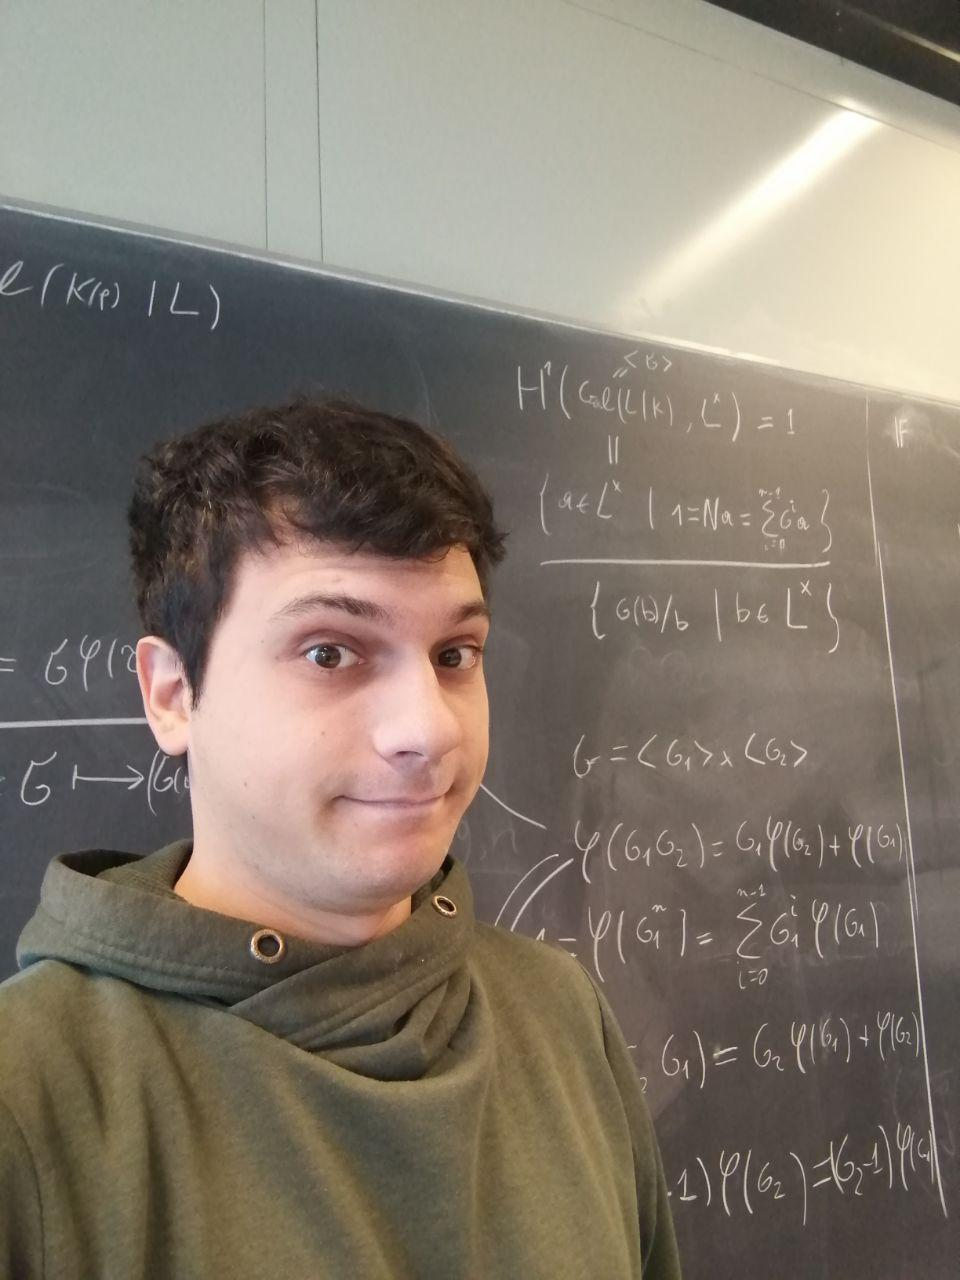
\includegraphics[height=3cm,angle=260]{me.jpg}
\caption{Me, upside-down}
\end{wrapfigure}

\lipsum

x \hfill y

Name: \hrulefill \quad Address: \dotfill

{\color{red} \lipsum }


\end{document}